%% beamer packages
% other themes: AnnArbor, Antibes, Bergen, Berkeley, Berlin, Boadilla, boxes, 
% CambridgeUS, Darmstadt, Dresden, Frankfurt, Goettingen, Hannover, Ilmenau,
%JuanLesPins, Luebeck, Madrid, Malmoe, Marburg, Montpellier, PaloAlto,
%Pittsburgh, Rochester, Singapore, Szeged, Warsaw
% other colors: albatross, beaver, crane, default, dolphin, dove, fly, lily, 
%orchid, rose, seagull, seahorse, sidebartab, structure, whale, wolverine,
%beetle

%\documentclass[xcolor=dvipsnames]{beamer}
\documentclass[table,dvipsnames]{beamer}
\usepackage{beamerthemesplit}
\usepackage{bm,amsmath,marvosym}
\usepackage{listings,color}%xcolor
\usepackage[ngerman]{babel}
\usepackage{natbib}
\usepackage[utf8]{inputenc}
\definecolor{shadecolor}{rgb}{.9, .9, .9}
\definecolor{darkblue}{rgb}{0.0,0.0,0.5}
\definecolor{myorange}{cmyk}{0,0.7,1,0}
%\definecolor{mypurple}{cmyk}{0.5,1.0,0,0.2}
\definecolor{mypurple}{cmyk}{0.3, 0.9, 0.0, 0.2}

% make a checkmark
\usepackage{tikz}
\def\checkmark{\tikz\fill[scale=0.4](0,.35) -- (.25,0) -- (1,.7) -- (.25,.15) -- cycle;} 

% dot product
\usetikzlibrary{arrows,positioning}
\tikzset{
    %Define standard arrow tip
    >=stealth',
    % Define arrow style
    pil/.style={->,thick}
}

% math stuff
\newcommand{\argmin}{\operatornamewithlimits{argmin}}

\lstnewenvironment{code}{
    \lstset{backgroundcolor=\color{shadecolor},
        showstringspaces=false,
        language=python,
        frame=single,
        framerule=0pt,
        keepspaces=true,
        breaklines=true,
        basicstyle=\ttfamily,
        keywordstyle=\bfseries,
        basicstyle=\ttfamily\scriptsize,
        keywordstyle=\color{blue}\ttfamily,
        stringstyle=\color{red}\ttfamily,
        commentstyle=\color{green}\ttfamily,
        columns=fullflexible
    }
}{}

\lstnewenvironment{codeout}{
    \lstset{backgroundcolor=\color{shadecolor},
        frame=single,
        framerule=0pt,
        breaklines=true,
        basicstyle=\ttfamily\scriptsize,
        columns=fullflexible
    }
}{}

\hypersetup{colorlinks = true, linkcolor=darkblue, citecolor=darkblue,urlcolor=darkblue}
\hypersetup{pdfauthor={A. Richards}, pdftitle={Support Vector Machines}}

\newcommand{\rd}{\textcolor{red}}
\newcommand{\grn}{\textcolor{green}}
\newcommand{\keywd}{\textcolor{myorange}}
\newcommand{\highlt}{\textcolor{darkblue}}
\newcommand{\norm}[1]{\left\lVert#1\right\rVert}
\def\ci{\perp\!\!\!\perp}
% set beamer theme and color
\usetheme{Frankfurt}
%\usetheme{Berkeley}
%\usecolortheme{dolphin}
\usecolortheme{seagull}
%\setbeamertemplate{blocks}[rounded][shadow=true]

\title[ARVoS]{Adaptive results visualization of sequences \\ ARVoS}
\author[]{Team-ARVoS}
\date[]{May 2017}

%%%%%%%%%%%%%%%%%%%%%%%%%%%%%%%%%%%%%%%%%%%%%%%%%%%%%%%%%%%%%%%%%%%%%%%%%%%%%%%
\begin{document}
\frame{\titlepage}
% %%%%%%%%%%%%%%%%%%%%%%%%%%%%%%%%%%%%%%%%%%%%%%%%%%%%%%%%%%%%%%%%%%%%%%%%%%%%%%%
% \frame{
% \footnotesize
% \tableofcontents
% \normalsize
% }

%%%%%%%%%%%%%%%%%%%%%%%%%%%%%%%%%%%%%%%%%%%%%%%%%%%%%%%%%%%%%%%%%%%%%%%%%%%%%%%
\frame{   
\frametitle{Principal Objectives}
\footnotesize
\begin{block}{Motivation}
 \begin{enumerate}
  \item Create a dynamic and interactive results display environment (Flask)
  \begin{itemize}
  \footnotesize
   \item Include both associative and \highlt{predictive} statistics
  \end{itemize}
  \item Create an environment that encourages model comparison
 \end{enumerate}
\end{block}  

 \begin{itemize}
  \item Apply it to a meta-analysis of asthma (reference assemblies) 
  \item Apply it to a \textit{de-novo} assembly from a unpublished butterfly species
  \item Create nice documentation using Sphinx
  \item Dockerize the databases and WebApp for ease of use
 \end{itemize}

}


%%%%%%%%%%%%%%%%%%%%%%%%%%%%%%%%%%%%%%%%%%%%%%%%%%%%%%%%%%%%%%%%%%%%%%%%%%%%%%%
\frame{
\frametitle{What we are not doing...}
\scriptsize
 \begin{center}
    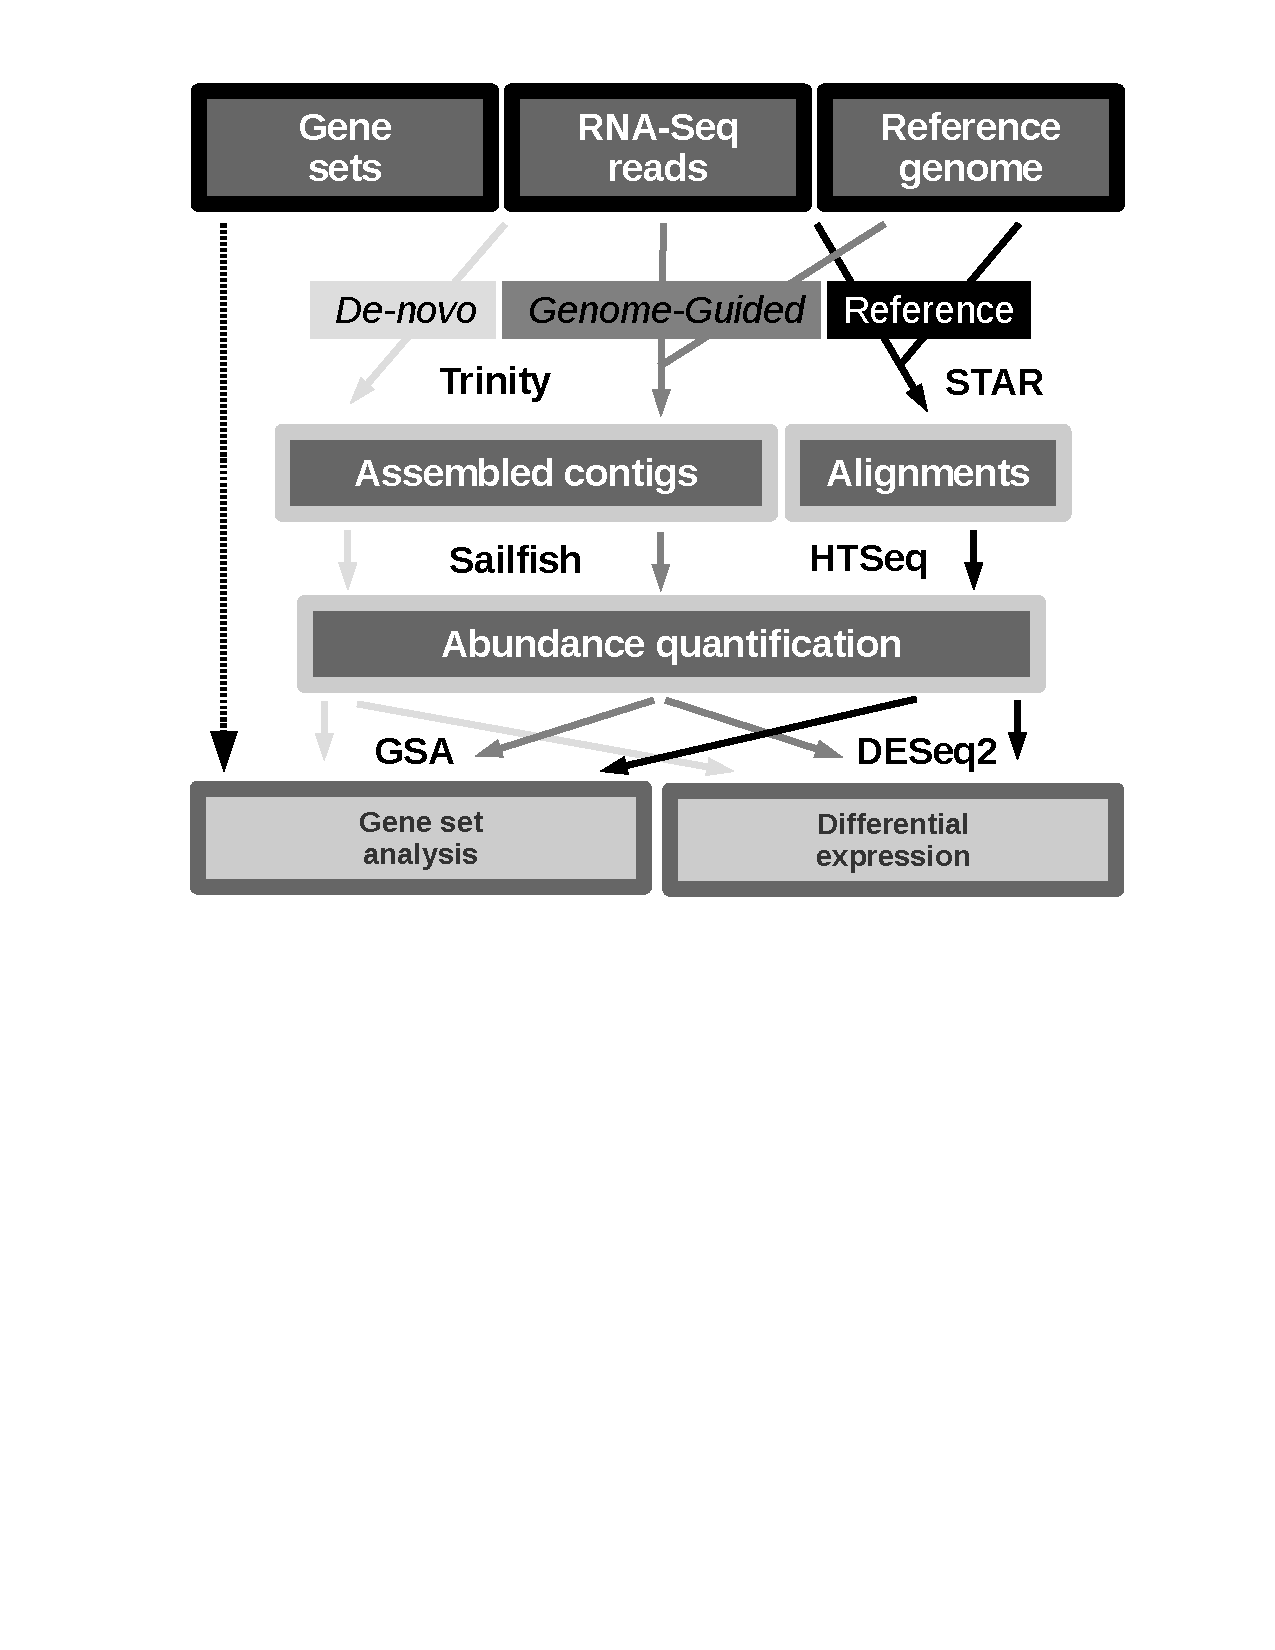
\includegraphics[scale=0.45]{expression-pipeline.pdf}  
 \end{center} 
}

%%%%%%%%%%%%%%%%%%%%%%%%%%%%%%%%%%%%%%%%%%%%%%%%%%%%%%%%%%%%%%%%%%%%%%%%%%%%%%%
\frame{
\frametitle{What we ARE doing...}
\scriptsize
 \begin{center}
    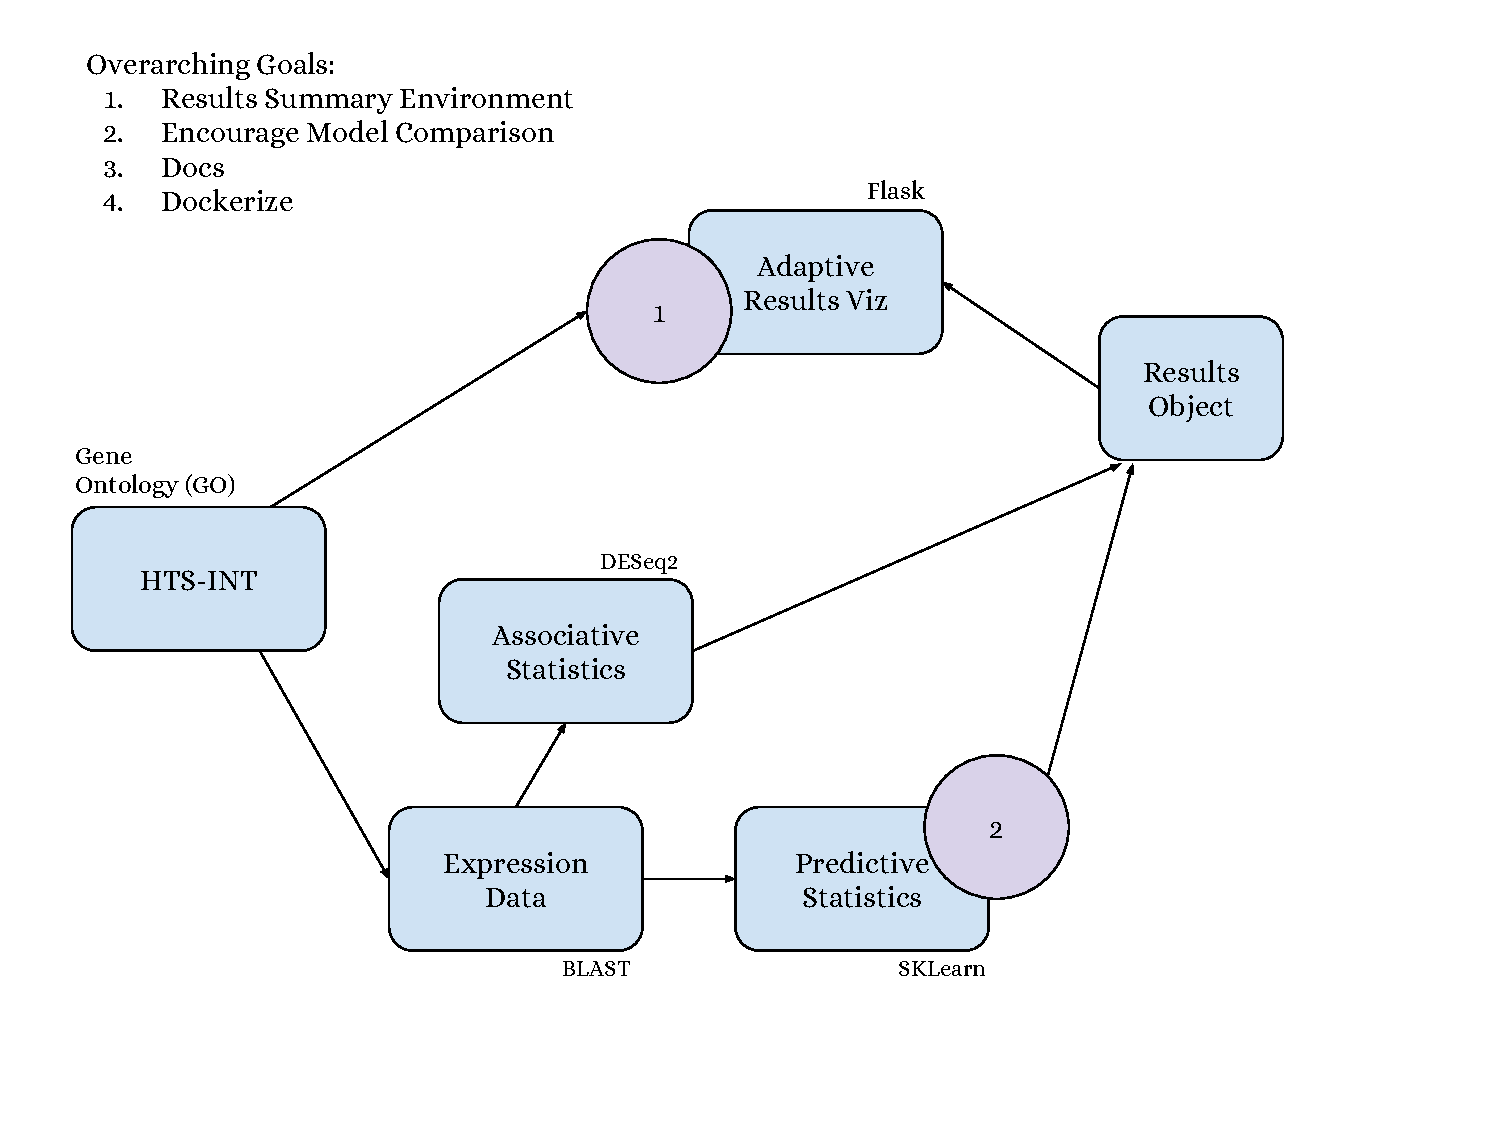
\includegraphics[scale=0.35]{game-plan.pdf}  
 \end{center} 
}

%   
% \begin{block}{Afternoon}
% \begin{itemize}
%   \item Python libraries and other tools / Datasets
%   \item Applications of community detection
%   \item Measuring quality of communities
%   \item Algorithms for dividing graphs into communities (Divisive, Agglomerative  
% \end{itemize}
% \end{block}
% }
% 
% %%%%%%%%%%%%%%%%%%%%%%%%%%%%%%%%%%%%%%%%%%%%%%%%%%%%%%%%%%%%%%%%%%%%%%%%%%%%%%%
%  \frame{ 
% \frametitle{Terms}
% \footnotesize
% 
%  \begin{center}
%     \includegraphics[scale=0.25]{edge-colormap.png}  
%  \end{center} 
% 
% \begin{itemize}
%  \item \highlt{network} and \highlt{graph} are used interchangeably
%  \item a graph is a set of \highlt{nodes} or vertices joined by lines or \highlt{edges}.
%  \item networks are all around us (roads, friendships, collaborations)
%  \item Provide a data structure that is intuitive 
% \end{itemize}
% }
% 
% %%%%%%%%%%%%%%%%%%%%%%%%%%%%%%%%%%%%%%%%%%%%%%%%%%%%%%%%%%%%%%%%%%%%%%%%%%%%%%%
%  \frame{ 
% \frametitle{NetworkX}
% \footnotesize
% \begin{itemize}
%   \item Python language data structures for graphs, digraphs, and multigraphs.
%   \item Many standard graph algorithms
%   \item Network structure and analysis measures
%   \item Generators for classic graphs, random graphs, and synthetic networks
%   \item Nodes can be "anything" (e.g. text, images, XML records)
%   \item Edges can hold arbitrary data (e.g. weights, time-series)
% \end{itemize} 
% 
% \begin{block}{}
% \tiny
% Originally developed by Aric Hagberg, Dan Schult, and Pieter Swart at Los Alamos National Laboratory, but now it is the main package to work with Network in Python and is developed by many others including Google.
% \end{block}
% 
% \begin{flushleft}
%  \tiny{\citep{Hagberg08}}
% \end{flushleft}
% }
% 
% %%%%%%%%%%%%%%%%%%%%%%%%%%%%%%%%%%%%%%%%%%%%%%%%%%%%%%%%%%%%%%%%%%%%%%%%%%%%%%%
%  \frame{ 
%  \frametitle{How to choose?}
%  \scriptsize
% \keywd{When to USE NetworkX to perform network analysis?}
% \begin{itemize}
%  \item Unlike many other tools, it is designed to handle data on a scale relevant to 
% modern problems.
%  \item Most of the core algorithms rely on extremely fast legacy code 
%  \item Highly flexible graph implementations (a graph/node can be anything!)
%  \item Extensive set of native readable and writable formats
%  \item Takes advantage of Python’s ability to pull data from the Internet or databases
% \end{itemize}
% 
% \keywd{When to AVOID NetworkX to perform network analysis?}
% \begin{itemize}
%  \item Large-scale problems that require faster approaches (i.e. Facebook/Twitter 
% whole social network...)
%  \item Better use of resources/threads than Python 
% \end{itemize}
% \begin{flushleft}
%  \tiny \href{https://www.cl.cam.ac.uk/~cm542/teaching/2010/stna-pdfs/stna-lecture8.pdf}{https://www.cl.cam.ac.uk/~cm542/teaching/2010/stna-pdfs/stna-lecture8.pdf}
% \end{flushleft}
% }
% 
% %%%%%%%%%%%%%%%%%%%%%%%%%%%%%%%%%%%%%%%%%%%%%%%%%%%%%%%%%%%%%%%%%%%%%%%%%%%%%%%
% \frame{ 
% \footnotesize
% \frametitle{Types of networks}
% \begin{center}
% \begin{tabular}{c|l}
% \hline
% Graph Type & NetworkX class \\
% \hline
% Undirected Simple & \texttt{Graph} \\
% Directed Simple & \texttt{DiGraph} \\
% With Self-loops & \texttt{Graph}, \texttt{DiGraph} \\
% With Parallel edges & \texttt{MultiGraph}, \texttt{MultiDiGraph} \\
% \hline
% \end{tabular}
% \end{center}
% }
% 
% %%%%%%%%%%%%%%%%%%%%%%%%%%%%%%%%%%%%%%%%%%%%%%%%%%%%%%%%%%%%%%%%%%%%%%%%%%%%%%%
% \frame{
% \frametitle{drawing and plotting}
% \scriptsize
% \begin{itemize}
%  \item Graphs are intuitive in part due to ease of visualization
%  \item It is possible to draw in graphs in:
%  \begin{itemize}
%   \item NetworkX 
%   \item GraphViz
%   \item matplotlib
%  \end{itemize}
% 
%  \begin{center}
%     \includegraphics[scale=0.25]{edge-colormap.png}  
%  \end{center} 
% Checkout the \href{https://networkx.github.io/documentation/development/gallery.html}{NetworkX Gallery} for some examples 
% \end{itemize}
% }
% 
% %%%%%%%%%%%%%%%%%%%%%%%%%%%%%%%%%%%%%%%%%%%%%%%%%%%%%%%%%%%%%%%%%%%%%%%%%%%%%%%
% \frame{
% \frametitle{Node and edge attributes}
% \begin{code}
% g.add_node(1, time='12AM') 
% print(g.node[1]['time'])
% print(g.node[1])
% \end{code}
% 
% \begin{code}
% g.add_edge(1, 2, weight=4.0 ) 
% g[1][2]['weight'] = 5.0 
% \end{code}
% }
% 
% %%%%%%%%%%%%%%%%%%%%%%%%%%%%%%%%%%%%%%%%%%%%%%%%%%%%%%%%%%%%%%%%%%%%%%%%%%%%%%%
% \frame{
% \frametitle{More terminology}
% \footnotesize
% 
% \begin{itemize}
%  \item \highlt{Neighbors}: The neighbors of a node are the nodes that it is connected to.
%  \begin{center}\texttt{G.neighbors(node)}\end{center}
%  \item \highlt{Degree}: The degree of a node is the number of neighbors for a given node 
%  \begin{center}\texttt{G.degree(node)}\end{center}
%  \item Directed graphs can be split into \highlt{indegree} and \highlt{outdegree}.
%  \begin{center}\texttt{DiGraph.in\_degree(node), DiGraph.out\_degree(node)}\end{center}
%  \item \highlt{Walk}: A walk is a sequence of nodes and edges that connect
%  \item \highlt{Path}: A path is a walk where no node is crossed twice 
%  \begin{center}\texttt{nx.shortest\_path(G)}\end{center}
%  \item A closed path is known as a \highlt{cycle} 
%  \begin{center}\href{https://networkx.github.io/documentation/networkx-1.10/reference/algorithms.cycles.html}{see the docs}\end{center}
% \end{itemize}
% }
% 
% %%%%%%%%%%%%%%%%%%%%%%%%%%%%%%%%%%%%%%%%%%%%%%%%%%%%%%%%%%%%%%%%%%%%%%%%%%%%%%%
% \frame{
% \frametitle{Even more terminology}
% \footnotesize
% \begin{itemize}
%  \item \highlt{Connected}: A graph is connected if every pair of vertices is connected by some path 
% \begin{center}\texttt{nx.is\_connected(G)}\end{center}
%  \item \highlt{Subgraph}: A subgraph is a subset of the nodes of a graph and all the edges between them
% \begin{center}\texttt{G.subgraph([0,1,2])}\end{center}
%  \item \highlt{Graph Diameter}: The diameter of a graph is the largest number of vertices that much be traversed in order to get from one vertex to any other vertex.
% \begin{center}\texttt{nx.diameter(G)}\end{center} 
% \end{itemize}
% }
% 
% %%%%%%%%%%%%%%%%%%%%%%%%%%%%%%%%%%%%%%%%%%%%%%%%%%%%%%%%%%%%%%%%%%%%%%%%%%%%%%%
% \frame{
% \frametitle{Resources}
% \begin{itemize}
%  \item \href{https://networkx.github.io/documentation/networkx-1.10/reference/algorithms.html}{NetworkX algorithms}
%  \item \href{https://www.cl.cam.ac.uk/teaching/1011/PrincComm/slides-lpr/graph_theory\_1-11.pdf}{graph theory tutorial}
%  \item \href{http://networkx.readthedocs.io/en/networkx-1.11/tutorial/tutorial.html}{NetworkX tutorial}
% \end{itemize}
% }

% 
% %%%%%%%%%%%%%%%%%%%%%%%%%%%%%%%%%%%%%%%%%%%%%%%%%%%%%%%%%%%%%%%%%%%%%%%%%%%%%%%
% \frame[allowframebreaks]{  
% \frametitle{References}
% \begin{tiny} \bibliography{../galvanize.bib}
% \bibliographystyle{apalike}         % Style BST file
% \end{tiny}
% }

\end{document}